\chapter{Modèle} \label{ch:modele}

Le modèle cherche à simuler la propagation de pandémies dans une population. Le système inclut un espace physique ainsi que des acteurs se déplaçant sur cette surface. Les acteurs sont des organismes vivants qui se déclinent en deux espèces distinctes. Le premier groupe fait partie des organismes victimes de l'épidémie et le second groupe est responsables de l'infection. Par conséquent nous sommes dans une situation ou une espèce en affecte une autre. Par contre dans le fonctionnement du modèle, il y a des restrictions sur la nature de l'espèce attaquante. Nous parlons ici d'organismes capables de contaminer un individu. \\

Les organismes évoluent dans un monde plat et parfaitement géométrique en deux dimensions. L'espace est comparable à un échiquier avec les acteurs étant des pions.

\section{Acteurs}

Il existe exclusivement deux espèces d'organismes dans le système :

\begin{enumerate}
	\item Les "agents pathogènes" sont les agents infectieux responsable de l'épidémie.
	\item Les "individus", éléments de la population victime de l'épidémie.
\end{enumerate}

La classe "agents pathogènes" ne fait pas référence à une espèce en particulier mais reflète des organismes avec le pouvoir d'infecter une autre espèce. Il peut s'agir de virus, bactéries ou encore de parasites. La caractéristique de ce groupe est qu'il a le pouvoir de rendre malade un individu et donc d'affecter une espèce par une maladie qu'il génère. Il peut s'agir de maladies touchant des humains ou de zoonoses suivant la nature des espèces du système. Le terme "pathogène" est aussi utilisé pour caractériser cette classe.\\

Les "Individus" sont les organismes susceptibles de développer la maladie suite à la contamination par un agent pathogène. Il peut s'agir d'humains tout comme d'animaux ou de plantes. La restriction est que cette espèce doit être affectée par les agents pathogènes ainsi que par la maladie.

\subsection{Individus}

Un individu peut se présenter sous deux formes distinctes. Il est soit sain, soit contaminé par un agent pathogène.\\

\begin{enumerate}
	\item La première forme décrit un individu qui n'est pas contaminé par un agent pathogène et donc n'est pas touché par la maladie.
	\item La seconde état survient lorsque l'individu est contaminé par un agent pathogène. Le modèle ne fait pas la distinction entre malade et porteur du pathogène, la notion de malade n'est pas prise en compte. Un individu infecté par un agent pathogène est contagieux, ce qui signifie qu'il a la pouvoir de transmettre l'agent pathogène à d'autres individus.
\end{enumerate}

\subsection{Agents pathogènes}

Un agent pathogène peut se présenter sous deux formes distinctes. Il est soit contaminant un individu, soit contaminant un espace physique.

\begin{enumerate}
\item Le premier cas est identique à celui précédemment développé mais cette fois ci, la situation est perçue du point de vue de l'agent pathogène. Quand un individu devient contaminé par un agent pathogène, ce dernier est absorbé par l'individu. C'est-à-dire que l'agent pathogène n'est plus une entité distincte mais fait partie intégrante de l'individu. Par conséquent l'individu sain devient un individu contaminé et non pas un individu sain associé à un agent pathogène.
\item Le second cas indique qu'une surface physique est contaminée par un agent pathogène. Un individu contaminé, en plus de contaminer d'autres individus sains, peut contaminer une surface. Si une surface est contaminée, une copie de l'agent pathogène de l'individu se dépose sur la surface. Un agent pathogène qui contamine une surface est inerte, c'est-à-dire qu'il ne peut pas se déplacer ni muter par contre il a toujours le potentiel de contaminer des individus sains qui se trouveraient sur cette surface. Un agent pathogène isolé sur une surface ainsi n'a une durée de vie que très limitée. Sa chance survie est paramétrable dans le modèle.
\end{enumerate}

\section{Espace physique}

L'espace physique est une surface plane sur laquelle on peut placer et déplacer des acteurs. La surface se présente sous la forme d'une grille régulière tel un échiquier. Cette grille est constituée de cellules dans lesquelles on peut y placer des acteurs. Cet espace bidimensionnel est la seule représentation spatiale du modèle. Chaque acteur a des coordonnées dans cet espace qui définissent sa position. Par conséquent, chaque cellule de la grille est indexée par une paire d'entiers.

\subsection{Cellule}

Dans la représentation du modèle, une cellule n'a que $6$ états possibles, c'est-à-dire que chaque cellule de la grille ne peut se retrouver que dans $6$ configurations différentes. L'état d'une cellule fait référence à l'acteur ou aux acteurs qui s'y trouvent. Concrètement une cellule est simplement une surface carrée mais nous associons les acteurs se trouvant sur la cellule à cette dernière et ceci décrit son état. Les $6$ états possibles d'une cellule sont listés ci-dessous.

\begin{enumerate}
	\item La cellule est vide, aucun acteur ne l'occupe. Cette situation signifie simplement que la surface n'est occupée par aucun acteur et est libre pour en accueillir un.
	\item Un individu sain se trouve sur la cellule.
	\item Un individu infecté se trouve sur la cellule.
	\item Un agent pathogène se trouve sur la cellule, infectant l'espace, sans individu.
	\item Un individu sain se trouve sur une cellule contaminée par un agent pathogène.
	\item Un individu contaminé se trouve sur une cellule déjà contaminée par un agent pathogène.
\end{enumerate}

Le cas $5$ et $6$ sont les deux seuls cas ou deux acteurs se trouvent simultanément sur la même cellule. Il est par conséquent impossible que deux individus se retrouvent sur la même cellule au même moment.

\begin{figure}[h]
	\centering
	\captionsetup{justification=centering}
	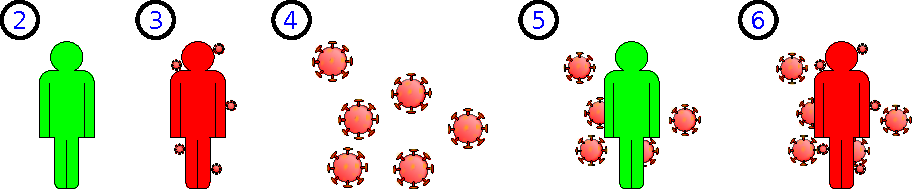
\includegraphics[scale=0.7]{Images/cell_states.pdf}
	\caption[Différents états de la cellule]{Une cellule possède différents états : (2) individu sain, (3) individu contaminé, (4) agent pathogène contaminant une cellule, (5) individu sain sur un espace contaminé, (6) individu contaminé sur un espace contaminé. Sans oublier l'état ou la cellule est vide.  }
\end{figure}

\newpage

\subsection{Grille régulière}

La grille régulière est l'espace sur lequel les acteurs évoluent. Chaque acteur est représenté au niveau spatial par ses coordonnées sur la grille et cette dernière leur permet de se déplacer et d'interagir. Les acteurs ne peuvent évoluer spatialement qu'en respectant la géométrie de la grille. Les bords du système sont périodiques, c'est-à-dire qu'un acteur n'est pas bloqué par un bord du système. Dans le cas où un individu souhaite se déplacer en dehors du système nous le faisons sauter à l'opposé de la grille. Les bords sont donc connectés afin d'éviter les effets de bords. \\

Un exemple de système en cours de simulation est illustré ci-dessous.

\begin{figure}[h]
	\centering
	\captionsetup{justification=centering}
	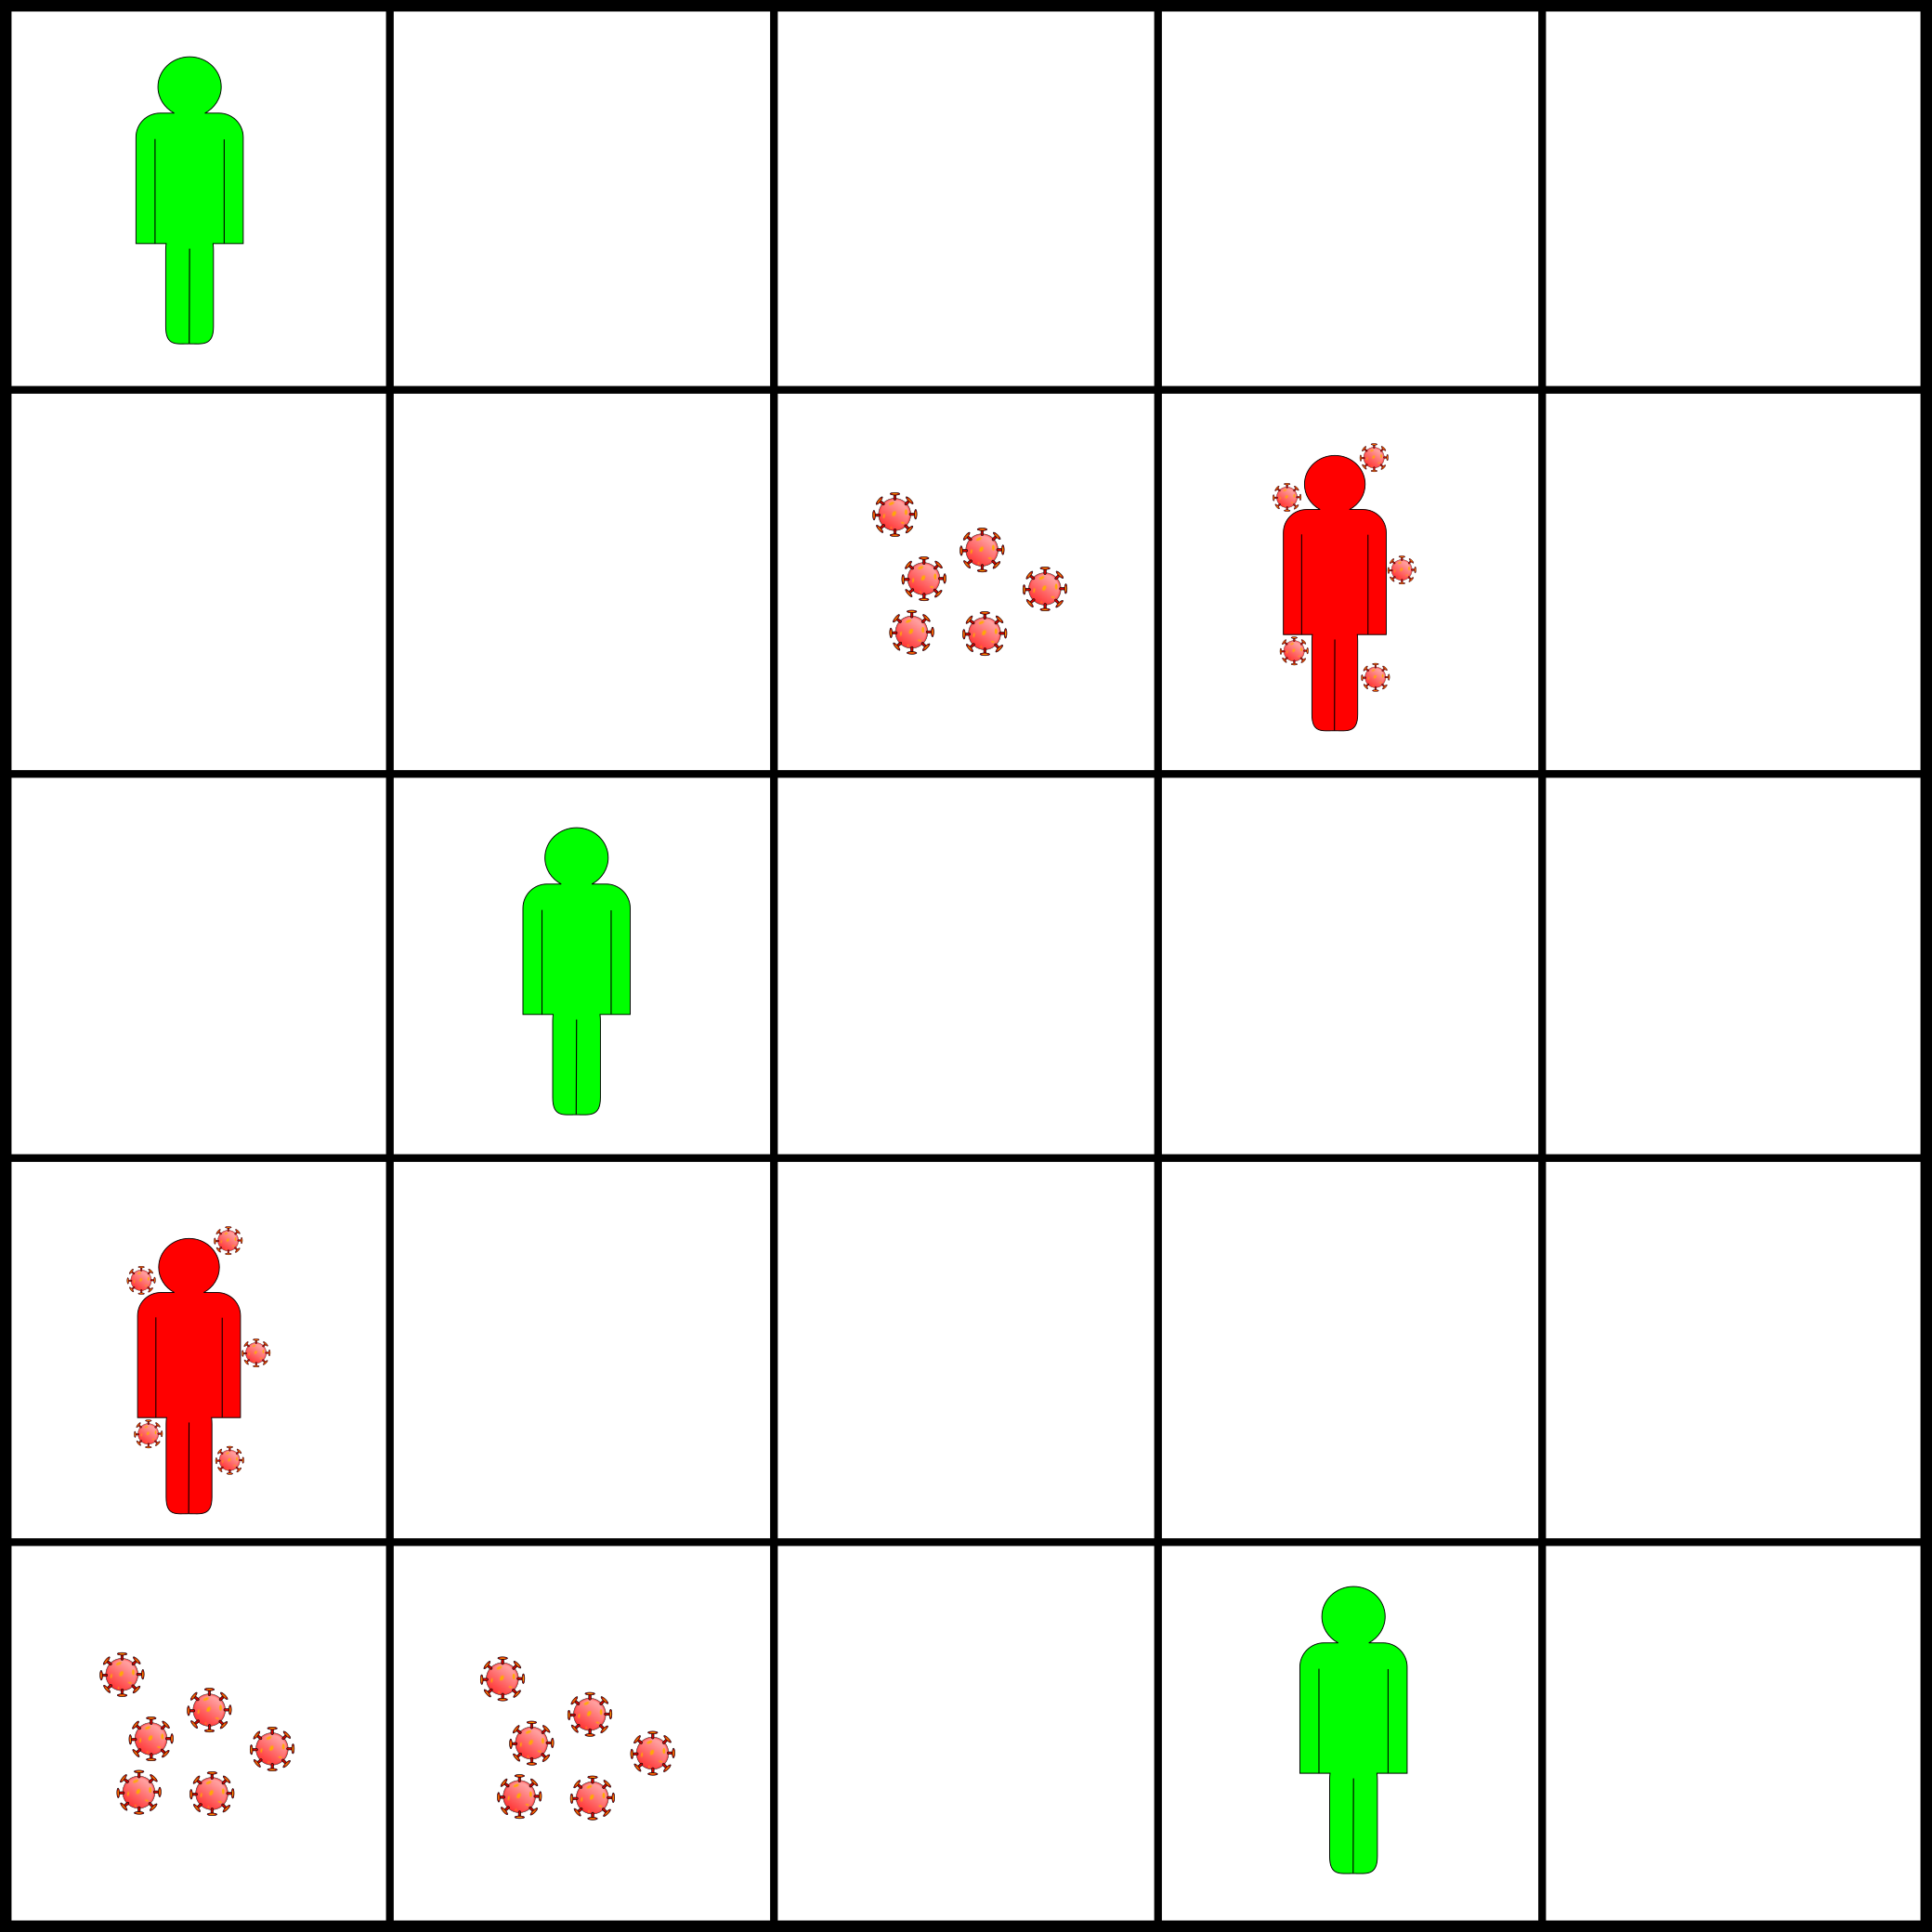
\includegraphics[scale=0.5]{Images/grid.png}
	\caption[Grille régulière]{Exemple d'une simulation en cours avec une grille de $5\times 5$ et $5$ individus.}
\end{figure}

L'espace bidimensionnelle permet de donner une représentation spatiale aux acteurs mais également de les faire interagir les uns avec les autres. Les interactions se font par la notion de voisinage.

\newpage

\subsection{Voisinage}

La représentation spatiale permet de situer tous les acteurs du système relativement les uns aux autres. Nous définissons que dans cet espace, les acteurs avec des coordonnées proches sont géographiquement rapprochés et peuvent s'influencer. Le voisinage est la transcription de cette proximité entre les acteurs et permet de définir la portée de l'influence des acteurs. Le voisinage d'une cellule est l'espace avoisinant à la cellule. Dans le modèle, le voisinage est représenté ainsi :\\

\begin{figure}[h]
	\centering
	\captionsetup{justification=centering}
	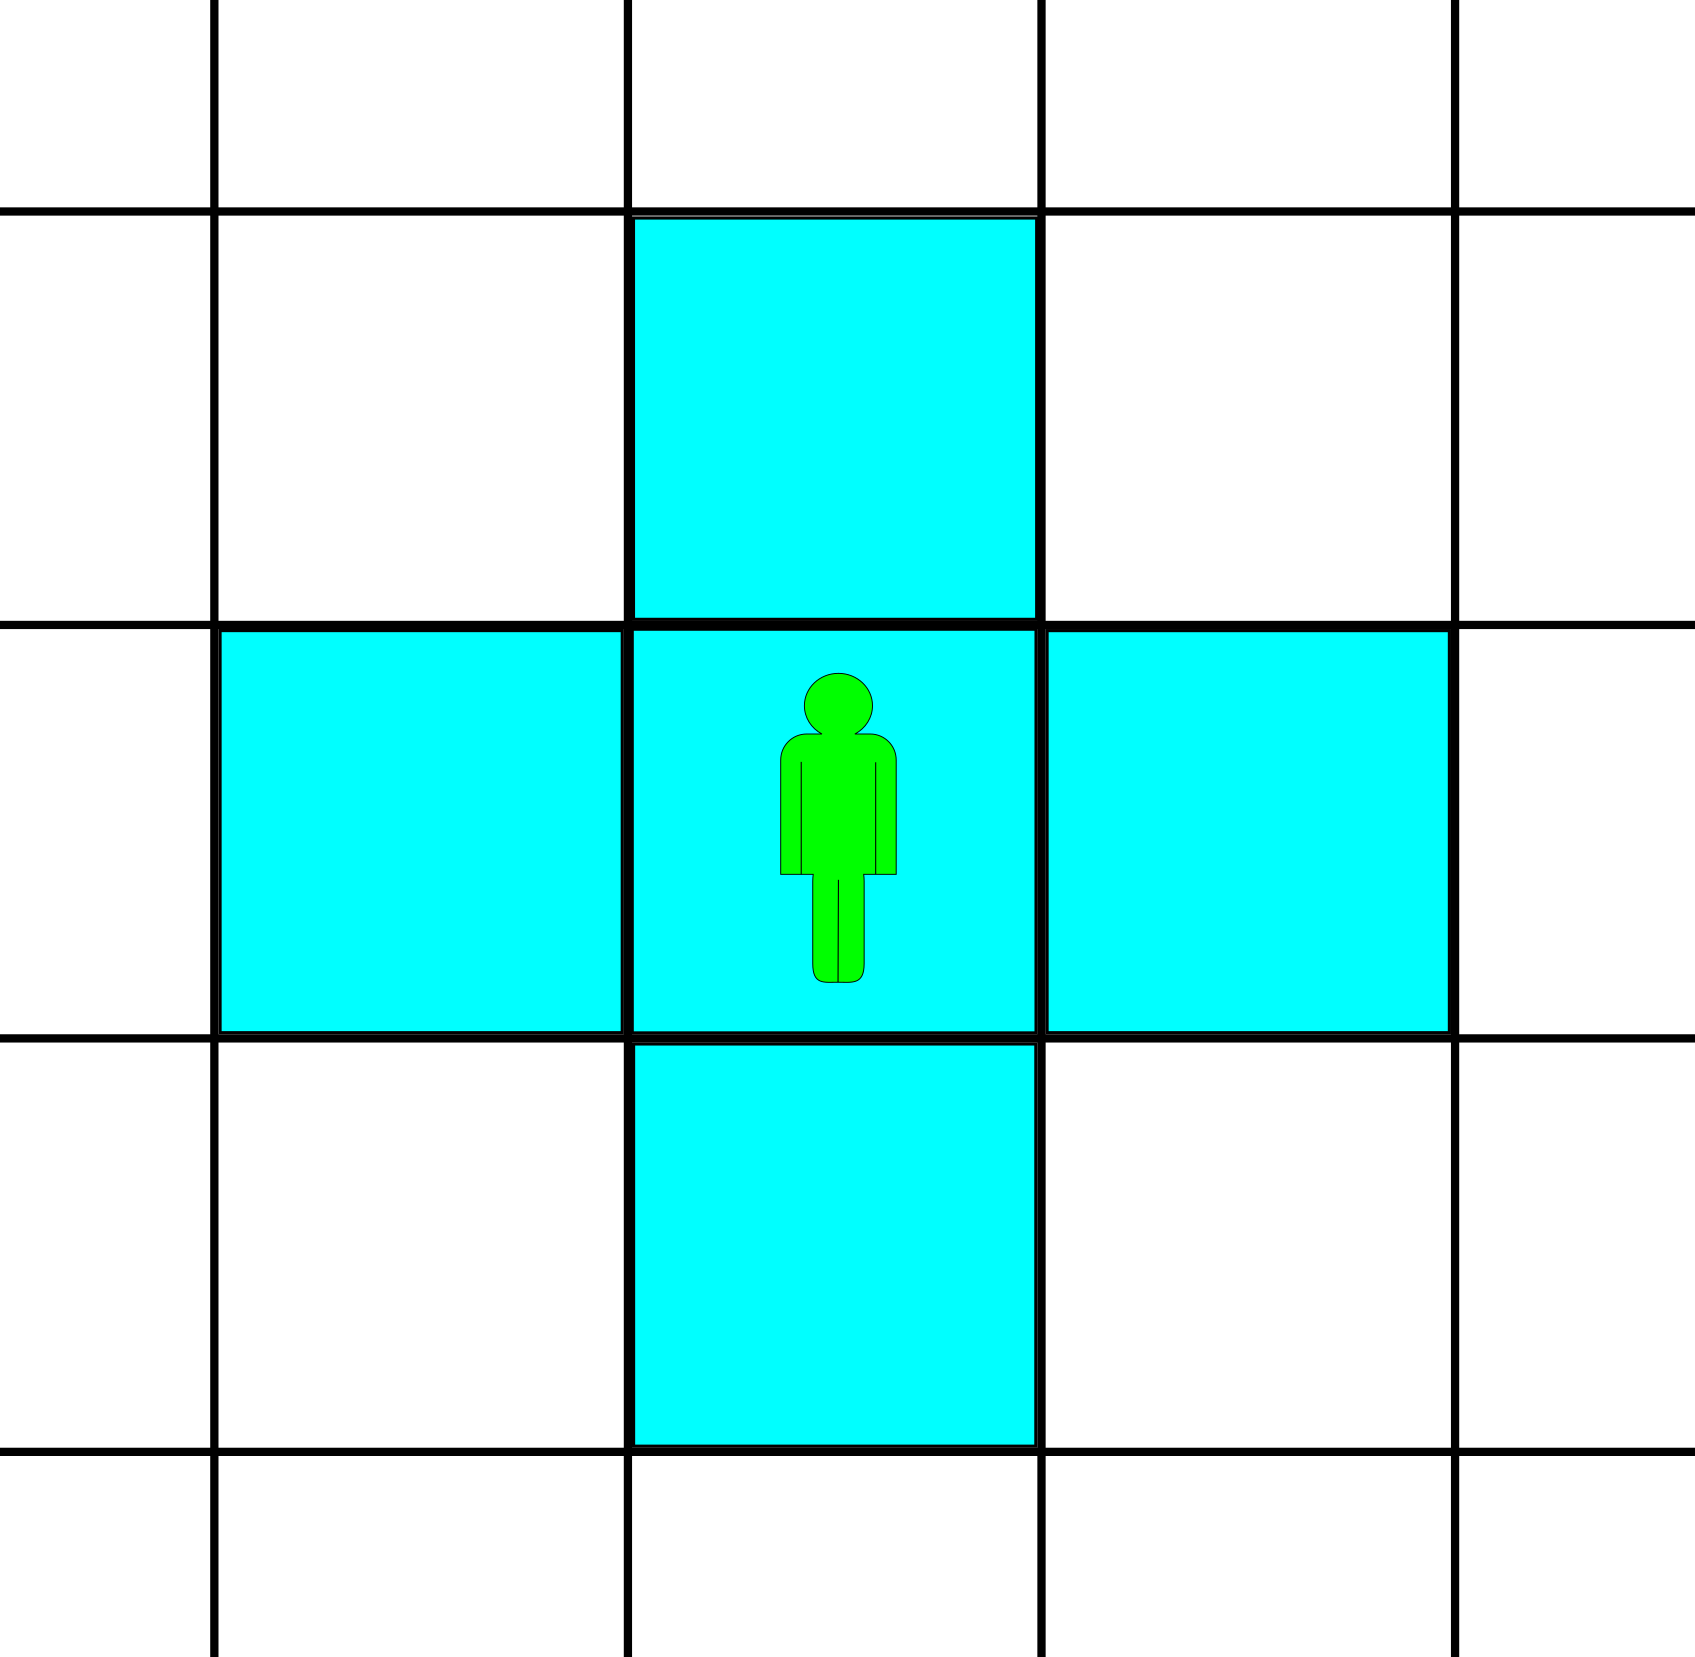
\includegraphics[scale=0.5]{Images/voisinage.png}
	\caption[Voisinage d'une cellule]{Le voisinage de la cellule centrale est les $4$ cellules en contact direct ainsi que la cellule centrale.}
\end{figure}

Le voisinage de la cellule contenant un acteur est les $4$ cellules avoisinantes directes en plus de la cellule centrale. Par conséquent notre humain dans cette cellule ne pourra interagir qu'avec des acteurs dans les cellules voisines (en cyan) ou avec un autre acteur sur sa cellule. Le reste du système lui est hors de portée et donc invisible. Par conséquent, les actions et l'état d'un acteur ne sont influencés que par son l'état actuel ainsi que par son voisinage. Toutes les autres cellules ainsi que leurs acteurs n'ont aucun impact sur l'individu étudié.

\section{Simulation}

Afin d'initialiser une simulation nous commençons par définir la taille de la grille et le nombre d'individus et nous contaminons un individu. Il existe une multitude d'autres paramètres définissant les comportements des différentes mécaniques de la simulation que nous expliquerons plus loin. Par conséquent, une situation initiale se présente toujours sous la forme ci-dessous. Notre population est saine, sauf un seul individu qui porte l'agent pathogène initial. C'est le point de départ de toute épidémie avec la contamination du premier individu, le patient zéro. Il s'agit ensuite d'observer la propagation ou non du pathogène initial. Un exemple de configuration initiale pourrait être : \\

\begin{figure}[h]
	\centering
	\captionsetup{justification=centering}
	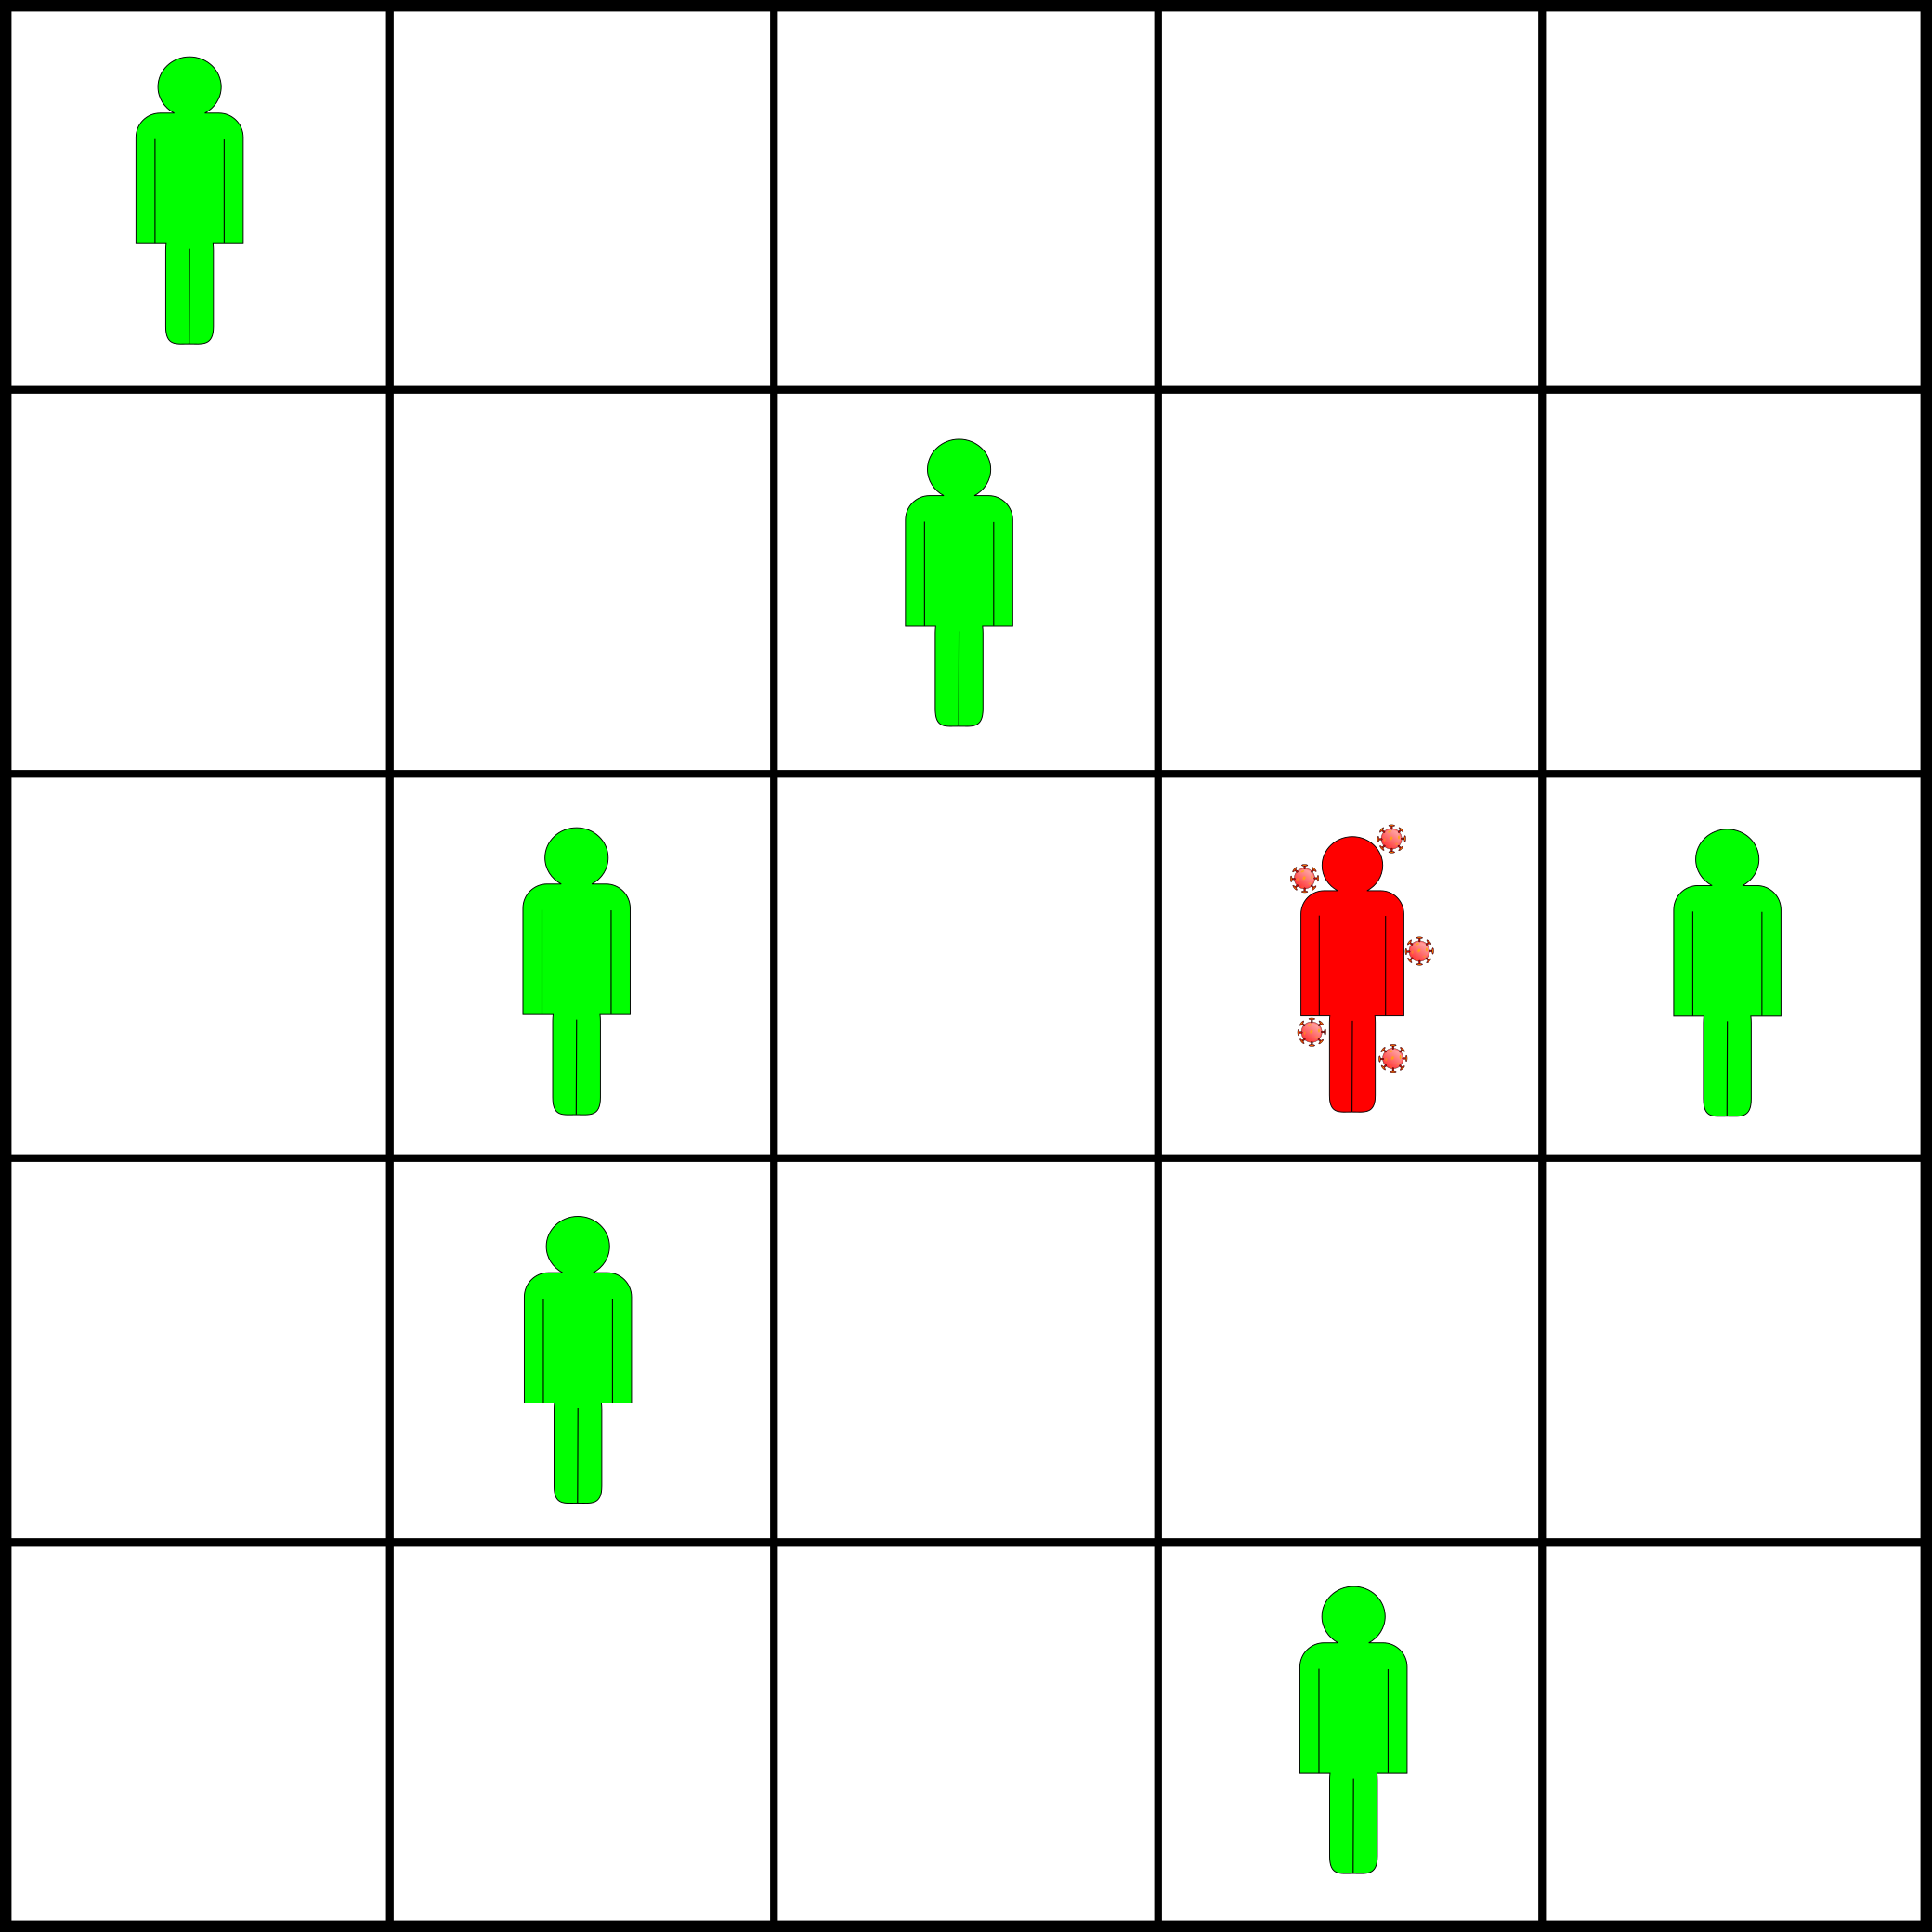
\includegraphics[scale=0.5]{Images/configuration_initiale.png}
	\caption[Configuration initiale]{Exemple d'une configuration initiale pour un système de taille $5\times 5$ avec $7$ individus.}
\end{figure}

Pour toutes configurations initiales, le placement des individus est aléatoire. A partir de là, un certain nombre d'itérations vont se produire permettant de faire évoluer le système.

\subsection{Itérations}

Depuis une configuration, le système peut évoluer par une itération. Une itération est une transition d'un état à un autre du système. Par exemple, depuis l'état initial de la simulation, donc l'état $0$ on peut passer à l'état $1$ par une transition qui est la première itération. Cette itération modifie les états de tous les acteurs et leur permet d'effectuer une ou plusieurs actions.\\

Pour être plus précis, une itération du système consiste en deux phases. La première est de mettre à jour tous les acteurs du système et la seconde est de permettre aux acteurs de se déplacer dans l'espace. La phase de mise à jour comprend l'actualisation de tous les acteurs ainsi que d'effectuer toutes les interactions entre les différents acteurs. La phase de mouvement permet uniquement aux individus de se déplacer sur la grille. Le détail de ces deux phases est explicité plus loin.\\

La simulation se termine après le déroulement d'un certain nombre d'itérations défini. La notion d'itération représente une certaine évolution dans le temps d'un système. C'est la seule représentation temporelle de la simulation.

\subsection{Mouvements des acteurs}

La phase de mouvement permet aux acteurs du système de physiquement se déplacer dans le domaine. Chaque acteur est sur une cellule caractérisée par des coordonnées et peut à cette phase bouger en changeant de cellule. Tous les acteurs ne peuvent pas se déplacer, seuls l'espèce "individu" peut se mouvoir. Les agents pathogènes ne peuvent pas se déplacer par eux-mêmes. Par conséquent, chaque individu peut se déplacer à chaque itération et ceci d'une seule cellule par déplacement. C'est-à-dire qu'un individu ne peut bouger que d'une cellule à la fois et ne peut pas se déplacer en diagonale. La portée de déplacement est illustrée ci-dessous et un individu a l'impossibilité de se déplacer sur une cellule si celle-ci est déjà occupée par un autre individu. Un paramètre du modèle permet d'effectuer plusieurs mouvements par itération, c'est-à-dire qu'un individu peut répéter $n$ fois ce processus de mouvement si le paramètre est fixé sur $n$.\\

\begin{figure}[h]
	\centering
	\captionsetup{justification=centering}
	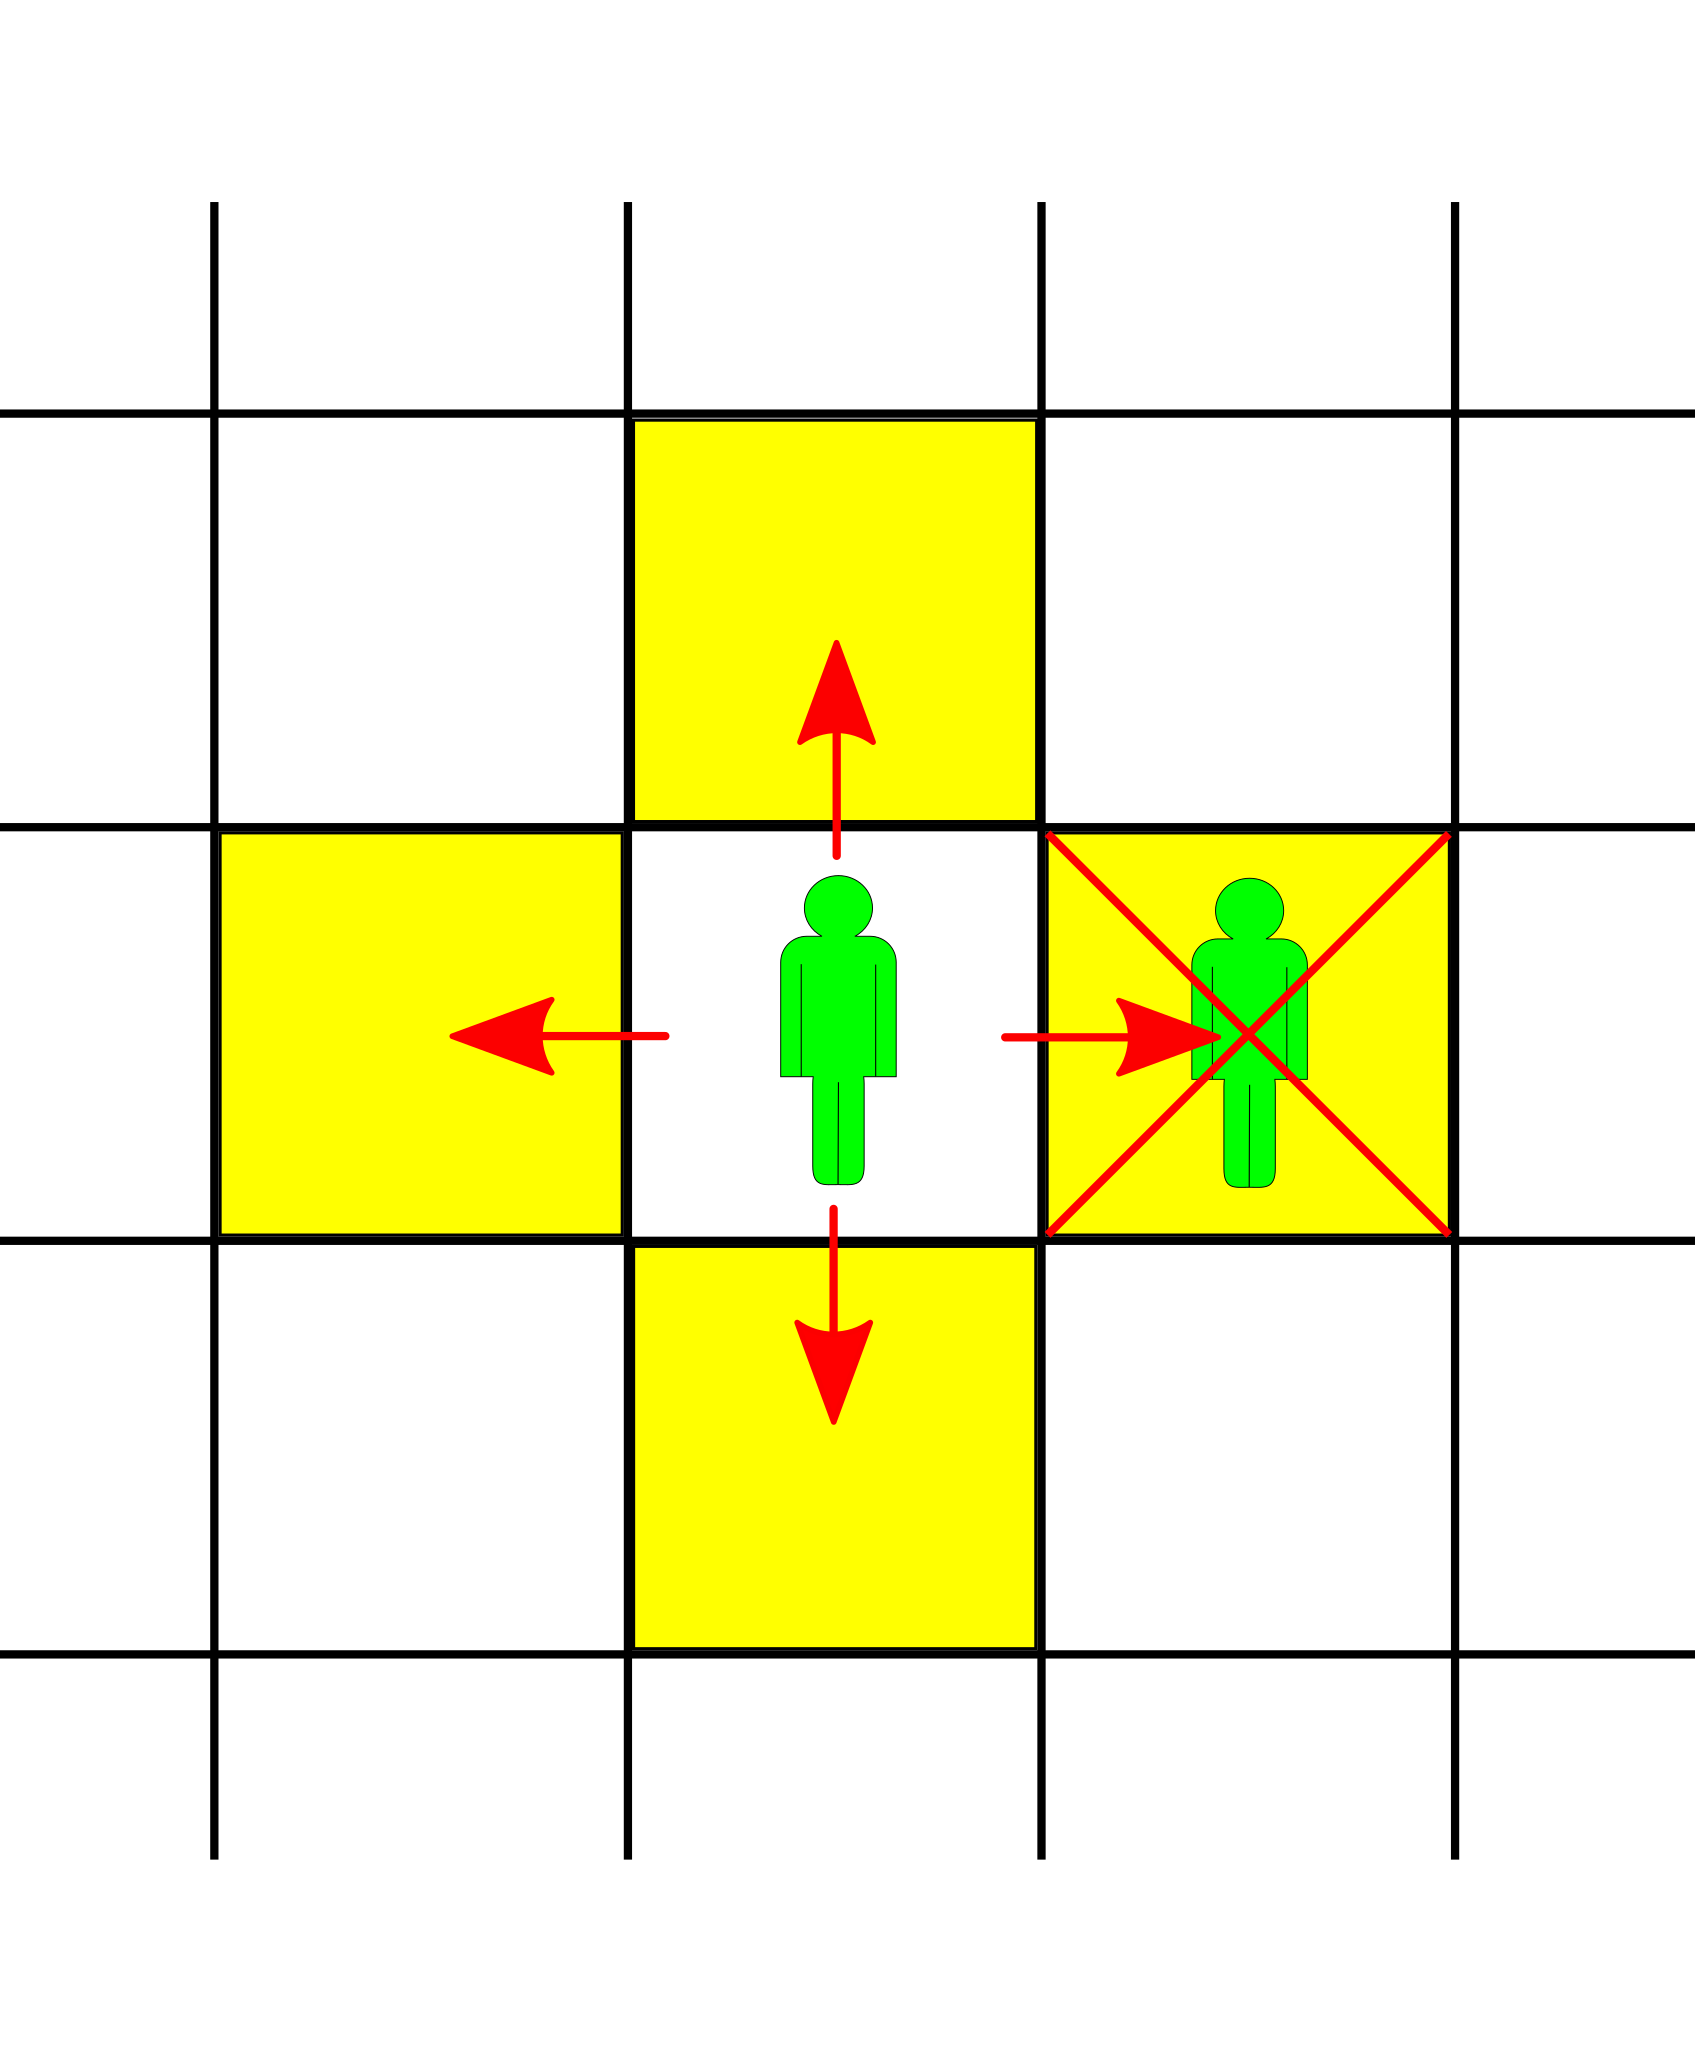
\includegraphics[scale=0.5]{Images/move_available.png}
	\caption[Mouvements des individus]{Lors d'un déplacement, un individu a $4$ choix possible (cellules en jaune) et en choisi un aléatoirement. Si la cellule sur laquelle l'individu veut aller est occupée alors il ne se déplace pas. Le processus peut être répété plusieurs fois par itération.}
\end{figure}

Sur cet exemple, l'individu sur la cellule centrale souhaite se déplacer. Sur les $4$ cases possibles pour un déplacement à cette itération, $3$ sont libres et $1$ occupée. Par conséquent notre humain ne peut pas se déplacer vers la droite. Le choix de l'individu pour le déplacement est aléatoire.\\

La procédure pour se déplacer est la suivante. Tout d'abord, l'individu choisit aléatoirement une des $4$ cellule voisine. Il vérifie ensuite que la cellule choisie soit libre. Si la cellule est libre il s'y déplace, sinon il ne bouge pas à cette itération et par conséquent reste là où il est. Une tentative non fructueuse de déplacement est quand même considérée comme déplacement, c'est-à-dire que si un individu se déplacer $5$ fois par itération mais est bloqué $2$ fois à cette itération alors il n'effectuera que $3$ réels déplacements.

\subsection{Mise à jour des acteurs}

\subsubsection{Actualisation des agents pathogènes}

Un agent pathogène peut se trouver dans deux états distincts. La procédure de mise à jour ne se produit que dans le cas où un agent pathogène contamine une cellule sans individu. Dans cette configuration sa survie est incertaine. Par conséquent il se peut que cet agent pathogène meurt. La phase de mise à jour de cet acteur sert à déterminer s'il meure à cette itération ou non.

\subsubsection{Actualisation des individus}

La procédure de mise à jour d'un individu dépend du fait qu'il soit infecté ou non.
\begin{enumerate}
	\item Dans le cas où l'individu mis à jour est sain, la seule étape à effectuer est l'analyse du voisinage. Cette phase consiste à regarder les cellules voisines et déterminer si l'individu finit contaminé ou non à cette itération. Une éventuelle contamination dépend exclusivement du voisinage. Si l'individu finit contaminer alors il intègre l'agent pathogène.
	\item Dans le cas où l'individu est déjà contaminé il est inutile d'analyser le voisinage. Par contre cet individu met à jour son état et ses attributs et ce processus a deux issues possibles.
	\begin{enumerate}
		\item Dans le premier cas, l'individu se débarrasse de son agent pathogène et redevient sain.
		\item Dans le second cas, l'individu conserve son agent pathogène ce qui laisse au pathogène la possibilité de muter.
	\end{enumerate} 
\end{enumerate}

Par conséquent, le système peut évoluer de deux manières différentes. Premièrement, les acteurs appartenant à l'espèce des individus peuvent se déplacent à chaque itération, modifiant leur position sur la grille. Deuxièmement les états de tous les acteurs du système peuvent changer grâce aux interactions entre acteurs mais aussi à l'actualisation de leurs attributs.\\

Les interactions se basent sur la notion de voisinage. Un acteur ne prend en considération durant sa mise à jour que les autres acteurs sur les cases voisines.

\section{Interactions}

Une interaction est une réaction réciproquer d'un acteur sur un autre. Les interactions se produisent entre les différents acteurs et permettent de faire évoluer le système. La première barrière à toutes interactions est la charge virale. La charge virale est un paramètre du modèle qui détermine la probabilité qu'une transmission soit possible entre deux acteurs. Autrement dit, il s'agit d'un facteur déterminant le niveau de contagion des agents pathogènes. Par conséquent, une faible charge virale signifie que les individus contaminés sont peu contagieux et ont donc peu de chance de transmettre leur agent pathogène en cas de contact. A l'opposé, une charge virale élevée signifie que les individus contaminés sont très contagieux et risquent de contaminer d'autres individus sains rapidement.\\

\subsection{Interactions sur la même cellule}

Le premier groupe d'interaction est celui des collisions d'acteurs sur la même cellule. Étant donné que deux individus ne peuvent pas se trouver sur la même cellule à la même itération, le seul cas à analyser survient lorsqu'un individu se trouve sur une cellule déjà contaminée par un agent pathogène. Il y a deux cas de collisions possible dans toutes simulations.

\begin{enumerate}
	\item Le premier cas se produit quand un individu sain se trouve sur une cellule déjà contaminée. Dans cette configuration, un individu sain se retrouve en contact direct avec un agent pathogène contaminant une cellule et risque donc d'être contaminé et de devenir l'hôte de cet agent pathogène.
	\item Le second cas se produit lorsqu'un individu contaminé se retrouve sur une cellule préalablement contaminée. L'agent pathogène contaminant la cellule n'a aucun impact sur l'individu car ce dernier est déjà l'hôte d'un autre agent pathogène. Par conséquent, les deux acteurs n'ont aucune influence l'un sur l'autre dans cette configuration.
\end{enumerate}

\subsection{Interactions sur cellules voisines}

Le deuxième type d'interactions se produit entre des acteurs qui sont spatialement proches mais sur des cellules différentes. Afin de permettre aux acteurs d'interagir sans être sur la même cellule, ils doivent appartenir à leur voisinage respectif. Seuls les individus peuvent effectuer ce type d'interactions. Par exemple, deux individus sur deux cellules adjacentes interagissent. Les différentes interactions possibles dans le modèle sont développées ci-dessous.

\begin{enumerate}
	\item Dans le cas où nous avons deux individus sains sur deux cellules voisines, l'interaction ne produit aucun résultat. Par conséquent, les individus n'ont pas d’impacts les uns sur les autres.
	\item Similairement au cas numéro $1$, si deux individus contaminés entrent en contact, aucune interaction ne se produit. Par conséquent, un individu contaminé n'a aucune influence sur un autre individu contaminé.
	\item Un cas plus intéressant survient lorsqu'un individu sain rentre en contact avec un autre contaminé. Lors de cette interaction il se peut que l'individu sain soit contaminé par l'individu contaminé. L'agent pathogène contenu dans l'individu contaminé pourrait avec une certaine probabilité se propager sur l'individu sain. Un individu sain peut donc être contaminé par un individu contaminé seulement si ce dernier se trouve dans son voisinage.
\end{enumerate}

\subsection{Contamination de cellule}

Une cellule est porteuse d'un agent pathogène si cet espace a été contaminé par un individu infecté. En effet, lorsqu’un individu infecté se déplace il a une certaine probabilité de contaminer l'espace qu'il occupait. Un paramètre fixe du modèle permet de déterminer cette probabilité. Une probabilité paramétrée élevée signifie que les individus contaminés infectent souvent les cellules qu'ils visitent et à l'inverse pour une probabilité faible.\\

Après un déplacement, l'individu contaminé à une certaine probabilité d'avoir contaminé la cellule qu'il occupait précédemment. Si la contamination a lieu, l'agent pathogène contaminant à présent la cellule est le même que celui contenu dans l'individu.\\

Un cas particulier peut se produire si un individu contamine un espace déjà contaminé par un autre agent pathogène. C'est-à-dire qu'un individu contaminé se trouvant sur une cellule préalablement contaminée et essaie de la contaminer à nouveau. Nous avons dit précédemment qu'un individu déjà infecté n'était pas sensible à un agent pathogène externe contaminant une cellule par contre il se pourrait que notre individu contamine lui aussi cette cellule. Dans ce cas précis nous écrasons l'agent pathogène initialement présent sur la surface et le remplaçons par une copie de l'agent pathogène de l'individu.

\section{Diversité génétique}

Le modèle se concentre sur la notion de diversité. Il faut donc un moyen pour représenter la diversité d'une population et gérer les interactions entre différents acteurs en prenant en considération leur diversité. La méthode utilisée se base sur des codes attribués à tous les acteurs du système. Chaque acteur possède un code et ce dernier simule son matériel génétique. Par conséquent, chaque individu et chaque agent pathogène possède un code que nous allons appeler "génome". Ce génome est un nombre entier non signé et se présente sous la forme d'une séquence codée sur $4$ octets. Nous avons dont $32$ bits disponibles afin de représenter le génome d'un acteur.\\

La notion de diversité d'une population peut à présent se définir par de grandes différences dans les génomes d'un individu à un autre. En effet, il y a une grande diversité au sein d'une population si les génomes des individus sont très différents les uns des autres. Le modèle intègre un paramètre permettant de définir le niveau de diversité des individus. L'unique agent pathogène initial n'a pas de notion de diversité, son génome est directement fixé dans les paramètres de la simulation.\\

La première étape de la génération de génomes est de commencer par attribuer à tous les individus un génome fixe et identique défini dans les paramètres de la simulation. Par conséquent, tous les individus ont ce même génome de référence, la diversité est nulle dans cette configuration. Il est ensuite possible de modifier ces génomes en complémentant un certain nombre de bits à partir de cette séquence de référence. Le processus de complémentation se fait aléatoirement et le nombre de complémentation dépend du paramètre de diversité du modèle. Par exemple, si le paramètre de diversité est défini à $5$ alors tous les individus effectueront $5$ modifications aléatoires sur leur séquence de référence. Etant donné que les changements sont aléatoires, les individus vont finir avec des génomes différents. Avec cette méthode nous finissons avec des génomes déviants plus ou moins d'un certain génome de référence.\\

Les génomes étant défini, il reste à définir la manière dont les agents pathogènes et les individus réagissent les uns avec les autres. Le problème est de savoir comment interpréter et utiliser des génomes. Comment gérer les comportements des acteurs en se basant sur des génomes de $32$ bits ? La technique utilisée est basée sur la distance de Hamming entre les séquences des génomes. Cette méthode fournit une solution permettant d'interpréter les génomes et de prendre des décisions. La principale utilité de cette interprétation survient avec les individus contaminés. Nous nous intéressons aux génomes afin de déterminer les compatibilités entre des individus et des agents pathogènes.\\

La distance de Hamming est une notion mathématique qui permet de calculer les différences entre deux séquences de symboles. Cette technique consiste simplement à compter le nombre de symboles différents pour deux suites de même longueur. Il s'agit donc de parcourir une des séquences et pour chaque indice comparer avec le symbole correspondant de l'autre séquence. Pour chaque symbole différent, la distance de Hamming est incrémentée de $1$.\\

Nous pouvons donc représenter la compatibilité entre un individu et un agent pathogène par cette distance sous forme d'un entier qui est la distance de Hamming entre les deux séquences. Il s'agit ensuite de convertir cette valeur en une probabilité. En effet, dans notre exemple il existe uniquement $33$ valeurs possibles de distances de Hamming qui caractérisent un match de génomes. Si nous définissons un seuil sur si peu de valeurs, les résultats vont être trop tranchés. Par conséquent nous convertissons cette distance calculée entre deux génomes en probabilité. Les actions à effectuer sont ensuite déterminée en fonction de cette probabilité.\\

\subsection{Distance de Hamming}

La distance de Hamming est un calcul s'effectuant sur deux séquences de symboles de même longueur. Il s'agit de quantifier la différence entre ces deux séquences par un entier. Un exemple sur deux séquences de $1$ octet est donné ci-dessous.

\begin{figure}[h]
	\centering
	\captionsetup{justification=centering}
	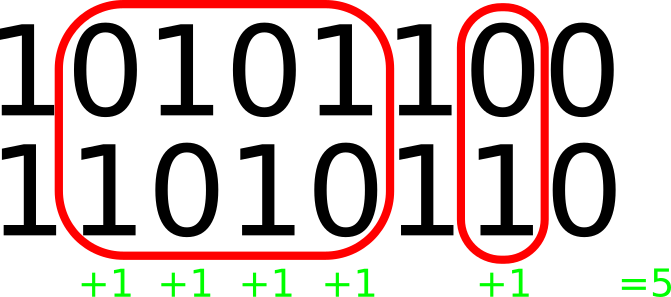
\includegraphics[scale=1]{Images/hamming.png}
	\caption[Calcul de la distance de Hamming]{Calcul de la distance de Hamming entre deux séquences binaires.}
\end{figure}

Dans cet exemple on peut voir en comparant les deux séquences de bits que sur $5$ positions les symboles diffèrent. Par conséquent la distance de Hamming entre la séquence $10101100$ et $11010110$ est égale à $5$.\\

Le calcul de la distance de Hamming s'effectue soit entre le génome d'un individu et celui d'un agent pathogène, soit entre deux agents pathogènes et détermine la compatibilité des deux organismes.\\

Le calcul de la distance de Hamming sert à déterminer si une action se déroule ou non. Il est donc nécessaire d'interpréter la distance de Hamming en lui donnant du sens. En effet, connaître la distance de Hamming entre deux génomes ne dit pas comment le système doit se comporter. Il faut traduire cette information en une forme utilisable. Un mécanisme de traduction produit une probabilité à partir d'une distance de Hamming. Nous aurions pu utiliser un seuil au-delà duquel l'action s'exécute. Au lieu de ce mécanismes, nous générons une probabilité reflétant cette distance et déterminant si l'action se produit ou non.\\

La distance de Hamming s’interprète de la manière suivante dans le modèle :

\begin{itemize}
	\item Une faible distance de Hamming donne l'ascendant à l'agent pathogène.
	\item Une grande distance de Hamming donne l'ascendant à l'individu.
\end{itemize}

L'idée principale est qu'un pathogène est efficace si son génome est "proche" de celui de l'individu qu'il attaque. Inversement l'agent pathogène est peu efficace si son génome est "éloigné" de celui de l'individu.\\

L'utilisation de la distance de Hamming ne survient principalement dans la situation ou un individu est déjà contaminé. Les individus contaminés, lors de leur mise à jour calculent la distance de Hamming qu'ils ont avec leur agent pathogène. Cette distance est ensuite traduite en probabilité et cette dernière détermine la chance qu'à les individus d'éliminer leur agent pathogène.\\

Hormis ce cas, le calcul de la distance de Hamming est aussi nécessaire lors de la gestion des immunités. Lorsqu'un individu rencontre un nouvel agent pathogène, il vérifie s'il est immunisé. Le même processus de probabilité est effectué pour déterminer si l'individu est immunisé ou non.

\section{Immunisation et résistance naturelle}

Le modèle intègre un principe d'immunisation et de résistance naturelle. Ces notions ne s'appliquent qu'aux organismes de l'espèce individu.\\

L'immunisation est une résistance acquise, c'est-à-dire qu'un individu contaminé a développé une immunité en présence d'un agent pathogène. C'est la situation ou l'individu reste contaminé un certain temps tout en contenant l'agent pathogène puis développe une immunité en combattant ce dernier. La notion de temps dans le modèle est donnée par les itérations, par conséquent si un individu reste contaminé pendant un certain nombre d'itérations puis finit par se débarrasser du pathogène alors il s'immunise.\\

Le mécanisme de résistance naturelle est identique au mécanisme d'immunisation, la seule différence est temporelle. Si un individu parvient à se débarrasser rapidement de son agent pathogène alors c'est une résistance naturelle. Par contre s'il faut davantage de temps, c'est une immunisation. Un paramètre du modèle définit le seuil en itérations découpant les deux processus. Par exemple, si le paramètre est défini à $5$ alors tous les individus qui parviennent à se débarrasser de leur agent pathogène en moins de $5$ tours (depuis leur contamination) sont considérés comme naturellement résistant. Les autres seront immunisés s'ils parviennent à éliminer le pathogène.\\

La particularité de l'immunisation est que le modèle intègre les immunités aux pathogènes sous la forme d'une liste d'attributs pour chaque individu. C'est-à-dire que chaque individu peut conserver des immunités aux pathogènes qui les ont contaminés. Deux méthodes permettant de déterminer l'immunité à partir de la liste d'attributs ont été implémenté est analysé dans le rapport. La première technique est la plus simple. Elle considère que les immunités des individus ne les protègent uniquement contre les agents pathogènes déjà rencontrés. Par exemple, si un individu développe une immunité contre un agent pathogène, l'individu ne sera plus affecté par ce génome d'agent pathogène dans le futur. Les individus du système ne peuvent pas développer des immunités à des groupes similaires de pathogènes, c'est des immunités au cas par cas. La seconde méthode qui est un peu plus élaboré fait appel à la distance de Hamming. Lorsqu'un individu rencontre un nouvel agent pathogène il contrôle ses immunités et pour chacune des immunités acquises effectue le calcul de la distance de Hamming entre le nouvel agent pathogène et l'immunité acquise afin de déterminer une probabilité d'être immunisé au nouveau pathogène. Par conséquent, un individu a de grandes chances d'être immunisé à un agent pathogène au génome proche d'un déjà rencontré.\\

Contrairement aux immunités, les résistances naturelles ne sont pas une réponse immunitaire. Par conséquent, les individus ne développent pas de résistance particulière aux agents pathogènes, ils sont "génétiquement" résistants. 

\section{Mutations}

Le modèle ne représente que des situations qui se déroule sur le court terme. C'est-à-dire que le temps d'une simulation à l'échelle de la vie d'un individu est assez faible. Par conséquent, les individus ne peuvent pas muter car nous estimons que durant toute la simulation, les individus ne changent pas de code génétique. Par contre les agents pathogènes peuvent évoluer rapidement. Ce sont les seuls acteurs à pouvoir muter dans le modèle.\\

Le modèle intègre un paramètre déterminant la probabilité qu'ont les agents pathogènes de muter à chaque itération. Seuls les agents pathogènes contaminant des individus peuvent muter. A chaque itération, l'individu essaie de se débarrasser de son agent pathogène. S'il échoue, le pathogène a la possibilité de muter. Une mutation se produit avec une certaine probabilité définie dans le modèle.\\

Une mutation est une modification du génome de l'acteur. Lorsqu'un agent pathogène mute il modifie un seul bit de sa séquence choisi aléatoirement. 